\section{Introduction}
Surface electromyography (sEMG) provides a non-invasive signal for gesture recognition and myoelectric control, but the recording interface must balance spatial information against the burden of additional electrodes \citep{scheme2011electromyogram,farina2014extraction,vujaklija2016new}. Fewer recording sites could simplify an interface. Whether that reduction preserves recognition for an unseen participant is an empirical question, and offline recognition alone does not establish a usable control interface.

Channel selection has been studied with feature filters, wrappers and spatial criteria \citep{phinyomark2012feature,stango2015spatial,qu2021reduce}. SHAP-guided EMG channel and feature optimization is also established \citep{rani2025shap}; related work uses Shapley explanations for similar sEMG gestures \citep{wang2024shap} and explainable feature selection with fusion \citep{gehlot2024fusion}. These contributions make attribution-based reduction a relevant comparator rather than a new algorithmic premise. Their performance estimates cannot be directly compared with this study across different tasks, sensors and validation protocols.

For a system intended to work across people, selection must exclude the eventual test participant. Using that participant to standardize features, estimate importance or choose a subset can produce optimistic estimates. Participant-disjoint inner evaluation also avoids measuring attribution solely on observations used to fit the attributing model. This motivates an outer leave-one-subject-out (LOSO) evaluation in which each entire selection procedure is reconstructed from the outer training participants.

Attribution magnitude describes predictive reliance of a fitted model, not a direct measurement of muscle activation. TreeSHAP distributes a model's prediction over its input features \citep{lundberg2017unified,lundberg2020local}; aggregation over an electrode's features offers a ranking, but does not turn it into a coalition-level Shapley value for that electrode. Correlated features and variation across participants can affect this ranking. Attribution stability has already motivated resampling and regularization methods \citep{visani2022statistical,xiang2026roshap}; a stability penalty therefore requires validation rather than a novelty claim.

Electrode count requires an explicit tolerance for performance loss. Non-inferiority asks whether a reduced system remains within such a tolerance, whereas a non-significant superiority test does not establish preservation \citep{schuirmann1987comparison,walker2011understanding}. A mean tolerance is also different from preserving every participant or gesture. Reporting only an aggregate curve could hide losses that matter to an intended application.

We evaluate cross-fitted electrode reduction on GRABMyo and separately examine NinaPro DB5. The primary question is the minimum count supported by a specified engineering margin. Secondary questions concern utility beyond random and spatial selection, stability regularization, and deletion with retraining. Exploratory analyses use a geometric subset under the primary training protocol, paired participant and gesture predictions, and shared-resource SHAP and grouped permutation rankings. Sensitivities and split-derived layouts delimit the claim: the LOSO experiment evaluates a selection procedure, not a prospectively validated common physical layout.

\begin{figure}[htbp]\centering
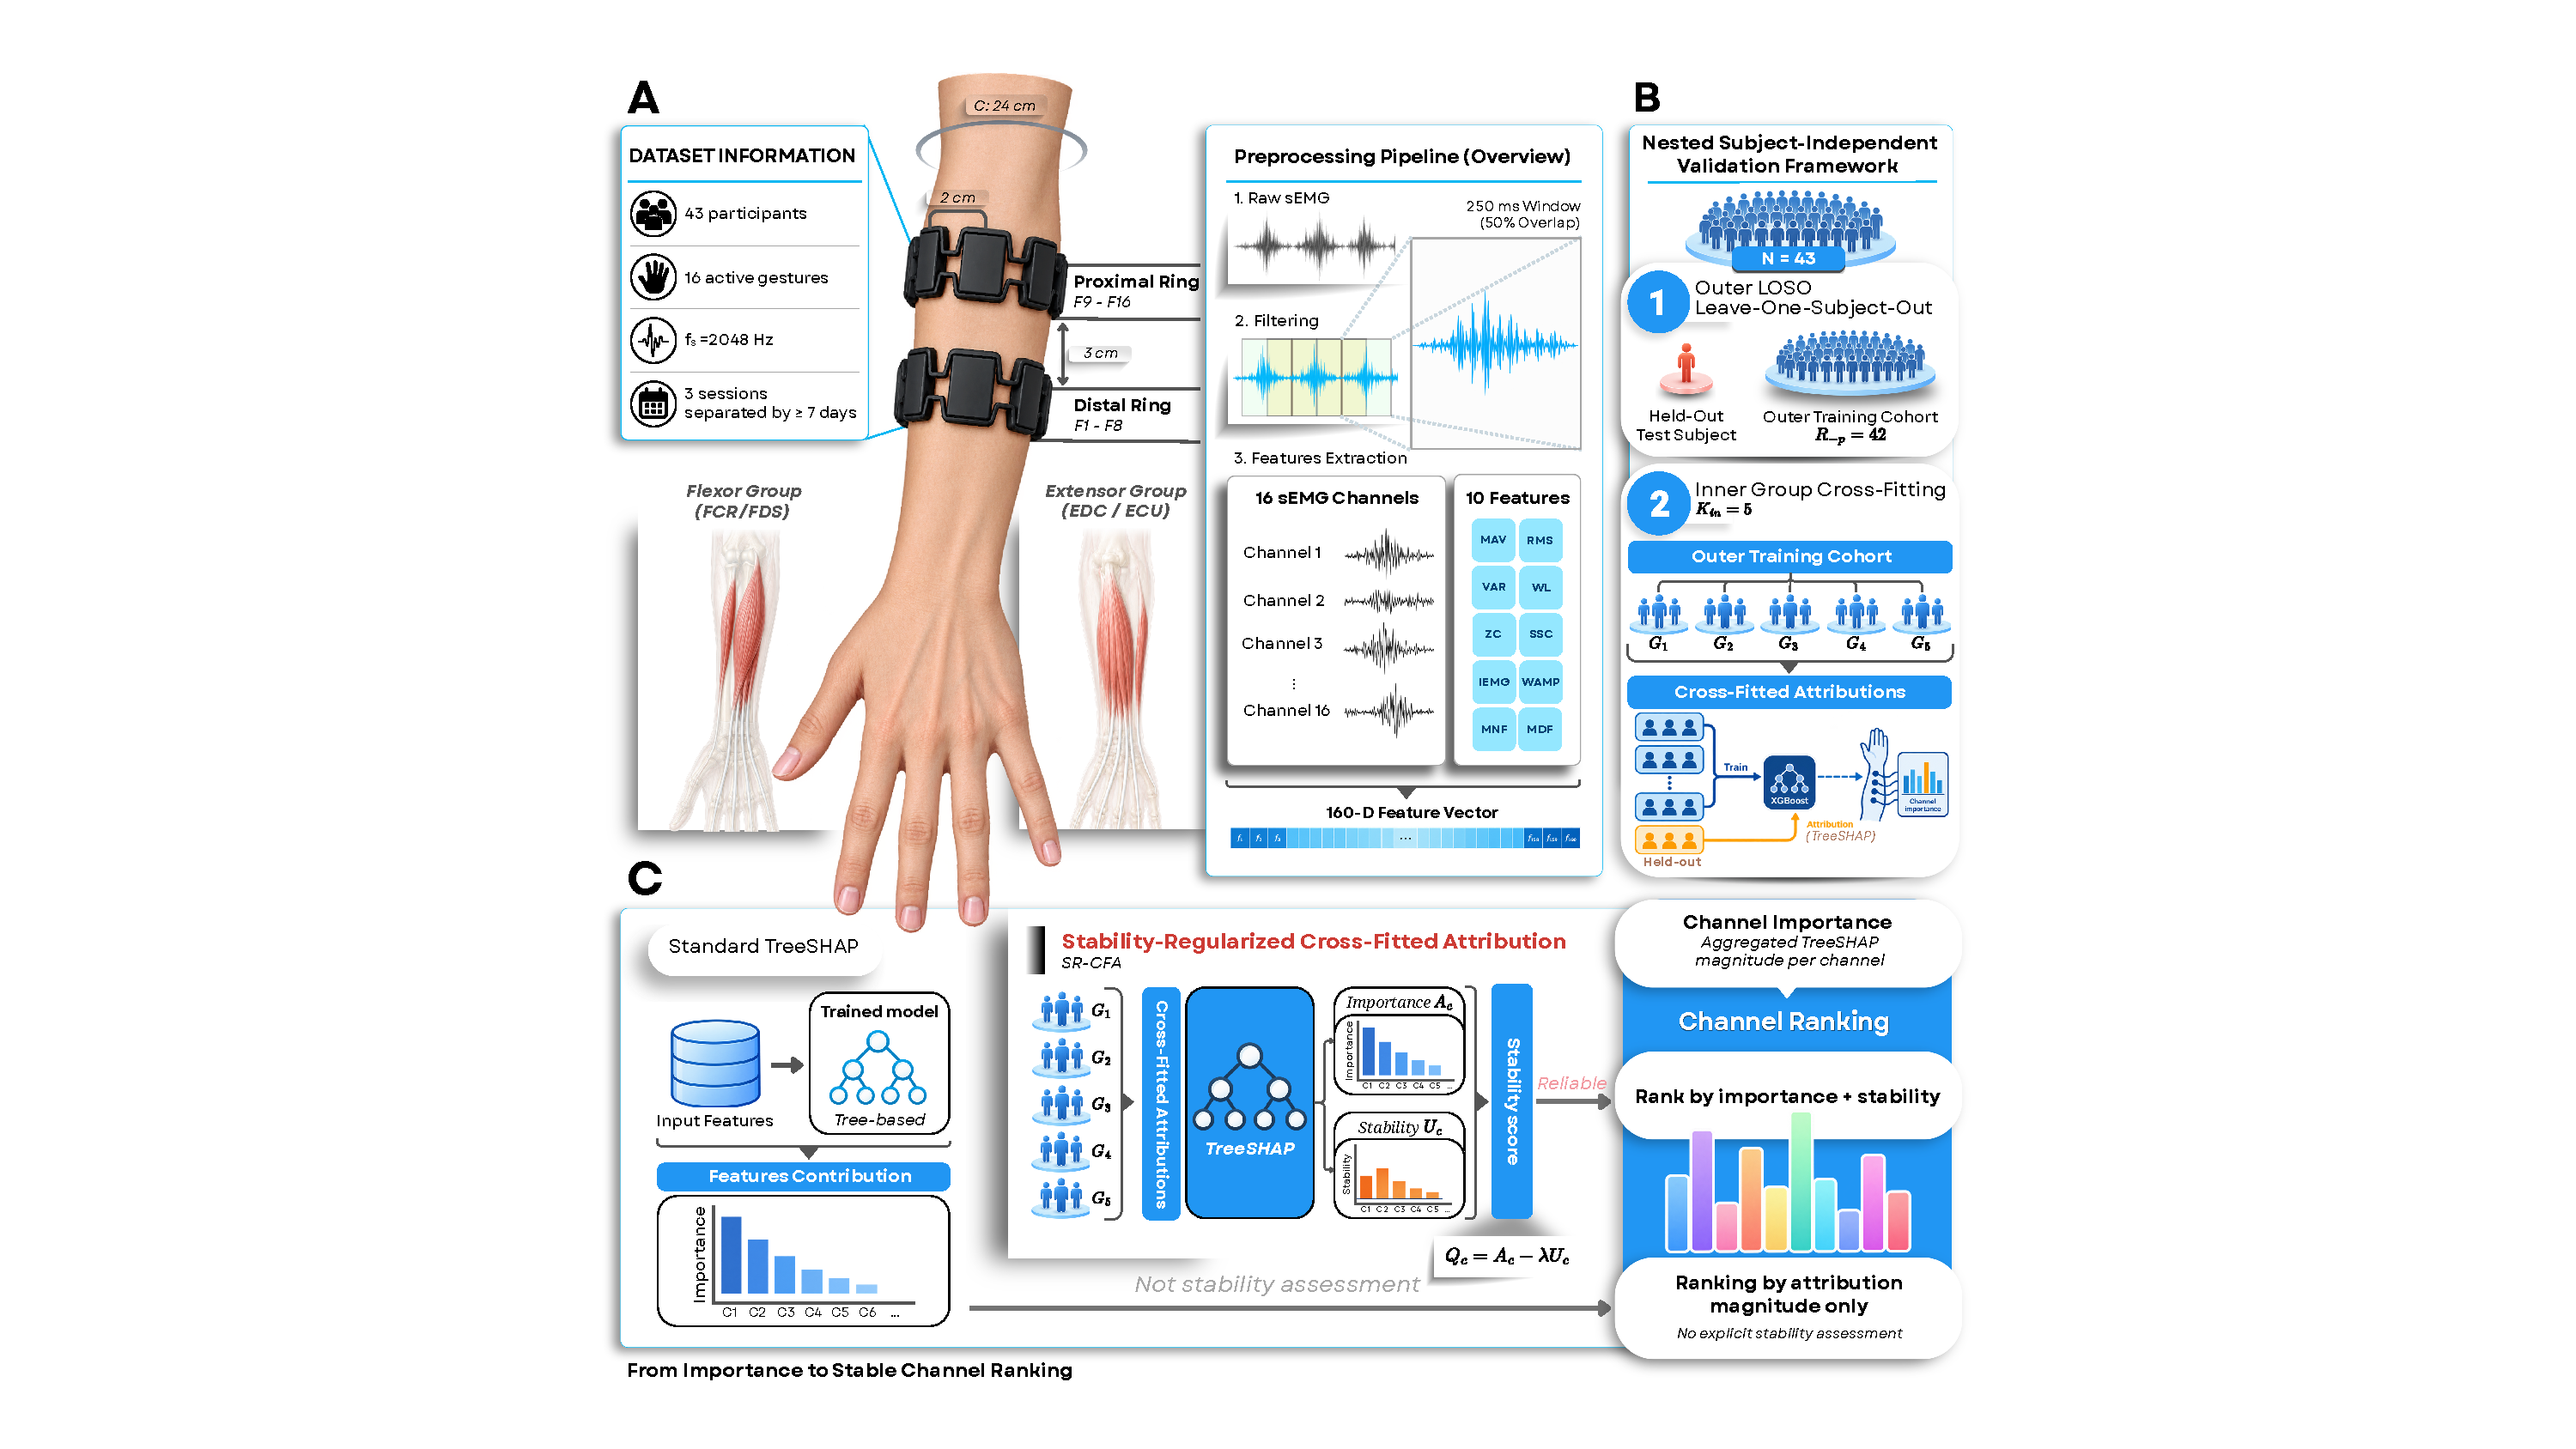
\includegraphics[width=\textwidth,trim=340bp 30bp 335bp 30bp,clip]{../figures/vector/fig1_montage.pdf}
\caption{Overview of the recording and selection procedure. (A) Forearm recording and feature extraction; the documented source montage comprises two aligned rings, with F1--F8 proximal and F9--F16 distal, separated by 2 cm. Anatomy, dimensions and waveforms in the artwork are illustrative; sites were not registered to individual muscles. (B) Outer participant-held-out evaluation and inner participant-grouped attribution. (C) Magnitude-only ranking and the fixed-penalty rule $Q_c=A_c-\lambda U_c$ evaluated in this study. The stability branch is a candidate procedure, not evidence that regularization improved recognition; numerical comparisons are reported in Results.}
\label{fig:montage}\end{figure}
